\chapter{STASE: statistics for malware datasets}
\label{chapter:stase}

\begin{quote}
{\itshape
There is generally a lack of consensus in antivirus engines' decisions on a given malware sample. This problem challenges the building of authoritative ground-truth datasets. Instead, researchers and practitioners may rely on unvalidated approaches to build their ground truth, e.g., by considering decisions from a selected set of antivirus vendors or by setting up a threshold number of positive detections before classifying a sample. Both approaches are biased, as they implicitly decide either on ranking antivirus products or on considering that all antivirus decisions have equal weights.
    
In this chapter, we extensively investigate the lack of agreement among antivirus engines. To that end, we propose a set of metrics that quantitatively describe the different dimensions of this lack of consensus. We show how our metrics can bring important insights by using the detection results of 66 AV products on 2 million Android apps as a case study. Our analysis focuses not only on antivirus binary decision but also on the notoriously hard problem of labels that antivirus associate with suspicious files, and allows to highlight biases hidden in the collection of a malware ground truth, a foundation stone of any machine learning-based malware detection approach.

\vfill

\begin{center}
On the Lack of Consensus in Anti-Virus Decisions: Metrics and Insights \\ on Building Ground Truths of Android Malware with VirusTotal

Médéric Hurier, Kevin Allix, \\ Tegawendé F. Bissyandé, Jacques Klein, Yves le Traon

13th Conference on Detection of Intrusions and \\ Malware \& Vulnerability Assessment (DIMVA) \\
July 6-8, 2016. San Sebastián, Spain

Source code: \url{https://github.com/fmind/stase}
\end{center}
}
\end{quote}

\localtableofcontents{}

To build ground truth datasets, antivirus engines appear to be the most affordable means today.
In particular, their application in research studies became more accessible thanks to online free services such as VirusTotal~\cite{noauthor_virustotal_nodate} that accepts the submission of any file for which it reports back the antivirus decisions from several vendors.
Unfortunately, antivirus engines disagree regularly on vetting malicious samples.
Their lack of consensus is observed in two dimensions: their binary decisions on the maliciousness of a sample are often conflicting and their labels are challenging to compare because of the lack of a standard for naming malware.

To consolidate datasets as ground truth based on antivirus decisions, researchers often opt to use heuristics that they claim to be reasonable.
For example, in the assessment of a state of the art machine learning based malware detection for Android~\cite{arp_drebin:_2014}, the authors have considered the reports from only ten antivirus engines, selected based on their popularity, dismissing all other reports.
They further consider a sample to be malicious once two antivirus engines agree to say so.
They claim that:

\begin{quote}
	This procedure ensures that [their] data is (almost) correctly split into benign and malicious samples—even if one of the ten scanners falsely labels a benign application as malicious~\cite[p.7]{arp_drebin:_2014}
\end{quote}

To gain some insights on the impact of such heuristics, we have built a dataset following these heuristics and another dataset following another typical process in the literature~\cite{kutylowski_droidminer:_2014}, which considers all antivirus reports from VirusTotal and accepts a sample as malicious as long as any of the antivirus flags it as such.
Furthermore, we propose a set of metrics for quantifying various dimensions of comparison for antivirus decisions and labels.
These metrics typically investigate to what extent the decisions of a given antivirus are exclusive with respect to other antivirus, or the degree of genericity at which antivirus vendors assign malware labels.

Our in-depth study of different heuristics parameters reveals discrepancies in the construction of ground truth datasets, and thus further question any comparison of detectors performance.
Similarly, the lack of consensus we observed in label naming prevents a proper assessment of the performance of detectors across malware families.
\section{Studying the impact of malware datasets}
\subsection{Dataset of Android applications and antivirus}
Our study leverages a large dataset of 2\,117\,825 Android applications and their analysis reports by 66 antivirus engines hosted by VirusTotal~\cite{noauthor_virustotal_nodate}.
\paragraph{Application dataset:}
We obtained our application samples by crawling popular application stores, including Google Play (70.33\% of the dataset), Anzhi (17.35\%) and AppChina (8.44\%), as well as via direct downloads (e.g., Genome - 0.06\%)~\cite{allix_androzoo:_2016}.
Table~\ref{table:stase:marketplaces} shows the distribution of Android applications across marketplaces.

\begin{table}[!ht]
    \caption{Distribution of applications by markets in our study}
    \label{table:stase:marketplaces}
    \centering
        \begin{tabular}{|c|r|r|}
        \hline
        \textbf{Marketplace} & \textbf{\# of Android applications} & \textbf{Percentage} \\
        \hline
        \texttt{Google Play} & 1\,489\,572 & 70.33\%\\
        \texttt{Anzhi} &  367\,534 & 17.35\%\\
        \texttt{AppChina} &  178\,648 & 8.44\%\\
        \texttt{1mobile} &  57\,506 & 2.72\%\\
        \texttt{AnGeeks} & 55\,481 & 2.62\%\\
        \texttt{Slideme} & 31\,681 & 1.50\%\\
        \texttt{torrents} & 5\,294 & 0.25\%\\
        \texttt{freewarelovers} & 4\,145 & 0.20\%\\
        \texttt{proandroid} & 3\,683 & 0.17\%\\
        \texttt{HiApk} & 2\,453 & 0.12\%\\
        \texttt{fdroid} &  2\,023 & 0.10\%\\
        \texttt{genome} &  1\,247 & 0.06\%\\
        \texttt{apk\_bang } & 363 & 0.02\%\\
        \hline
        \textbf{Total} & \textbf{2\,117\,825} & \\
        \hline
        \end{tabular}
\end{table}


\paragraph{Antivirus reports:}
We collected antivirus reports associated with our malware sets from VirusTotal~\cite{noauthor_virustotal_nodate}, an online platform that can test files against commercial antivirus engines.
For each application package file (APK) sent to VirusTotal, the platform returns, among other information, two pieces of information for each antivirus:

\begin{itemize}
	\item A binary flag (\texttt{True} = positive detection, \texttt{False} = negative detection)
	\item A string label to identify the threat (e.g., \texttt{Trojan:AndroidOS/GingerMaster.A})
\end{itemize}

Overall, we managed to obtain antivirus reports for 2\,063\,674 Android applications\footnote{we could not obtain the results for 54\,151 (2.56\%) applications because of a file size limit by VirusTotal}.
In this study, we explore those reports and define metrics to quantify the characteristics of several \emph{tentative ground truths}.
\subsection{Variations in experimental settings}
When experimenting with machine learning based malware detector, as it is nowadays common among security researchers, one of the very first steps is to build a ground truth, for training and also assessing the detector.
The question is then how to derive a ground truth based on antivirus reports of the millions of applications in existence.
In particular, we focus on which samples are considered as malicious and included in the malware set of the ground truth.
Based on methods seen in the literature, we consider the following three settings for building a ground truth:

\begin{itemize}
	\item \textbf{Baseline settings}: In these settings, we consider a straightforward process often used~\cite{allix_empirical_2016,kutylowski_droidminer:_2014} where a sample is malicious as long as any antivirus reports it with a positive detection. Thus, our ground truth with the Baseline settings and based on our 2 million applications, contains 689\,209 malware applications. These samples are reported by antivirus with 119\,156 distinct labels.

	\item \textbf{Genome settings}: In a few papers of the literature, researchers use for ground truth smaller datasets constituted of manually compiled and verified malicious samples. We consider such a case and propose such settings where the malware set of the ground truth is the Genome~\cite{zhou_dissecting_2012} dataset containing 1\,248 applications. Antivirus reports on these applications have yielded 7\,101 distinct labels.

	\item \textbf{Filtered settings}: Finally we consider a refined process in the literature where authors attempt to produce a clean ground truth dataset using heuristics. We follow the process used in a recent state-of-the-art work~\cite{arp_drebin:_2014}:
	      \begin{enumerate}
		      \item Use a set of popular antivirus scanners\footnote{antivirus considered in~\cite{arp_drebin:_2014}: AntiVir, AVG, Bit-Defender, ClamAV, ESET, F-Secure, Kaspersky, McAfee, Panda, Sophos}.
		      \item Select applications detected by at least two antiviruses in this set.
		      \item Remove applications whose label from any antivirus includes the keyword adware.
	      \end{enumerate}
	      With these settings, the malware set of the ground truth includes 44\,615 applications associated with 20\,308 distinct labels.
\end{itemize}

In the remainder of this chapter, we use $\mathcal{D}_{genome}$, $\mathcal{D}_{base}$, and $\mathcal{D}_{filtered}$ to refer to the three ground truth datasets.
The property of each dataset are summarized in Table~\ref{table:stase:experimental}, which includes the selection criteria and the final number of applications for each set.
We did not performed supplementary preprocessing besides the heuristics we mentioned in the previous paragraph to avoid potential biases in our study.

\begin{table}[!ht]
    \label{table:stase:experimental}
    \caption{Experimental ground-truth settings studied with STASE}
    \begin{tabular}{|c|c|c|c|c|}
    \hline
    & Initial Dataset & Genome dataset & Baseline dataset & Filtered dataset \\ \hline
    Notation & $\mathcal{D}^I$& $\mathcal{D}^G$& $\mathcal{D}^B $& $\mathcal{D}^D$\\% \hline
    Antivirus & 66 & 66 & 66 & 10 \\% \hline
    Applications & 2\,117\,825 & 1\,248	& 689\,209 & 	44\,615 \\% \hline
    Distinct labels & 119\,156 & 7\,101 & 	119\,156 & 	20\,308 \\% \hline
    Discard adware & No & No & No & Yes \\% \hline
    Threshold ($\tau$) & $\geq 0$& $\geq 0$& $\geq 1$& $\geq 2$ \\
    \hline
    \end{tabular}
\end{table}


\subsection{Notations and definitions}
Given a set of $n$ antivirus engines $\mathcal{A} = \{a_1, a_2, \cdots, a_n\}$ and a set of $m$ applications $\mathcal{P} = \{p_1, p_2, \cdots, p_m\}$, we collect the binary decisions and string labels in two $n \times m$ matrices denoted $\mathcal{B}$ and $\mathcal{L}$ respectively:

\[
	\mathcal{B} = \bordermatrix{ ~ & a_1 & a_2 & \ldots & a_n
		\cr p_1 & b_{1,1} & b_{1,2} & \ldots & b_{1,n}
		\cr p_2 & b_{2,1} & b_{2,2} & \ldots & b_{2,n}
		\cr \vdots & \vdots & \vdots & \ddots & \vdots
		\cr p_m & b_{m,1} & b_{m,2} & \ldots & b_{m,n} }
	%
	\mathcal{L} = \bordermatrix{ ~ & a_1 & a_2 & \ldots & a_n
		\cr p_1 & l_{1,1} & l_{1,2} & \ldots & l_{1,n}
		\cr p_2 & l_{2,1} & l_{2,2} & \ldots & l_{2,n}
		\cr \vdots & \vdots & \vdots & \ddots & \vdots
		\cr p_m & l_{m,1} & l_{m,2} & \ldots & l_{m,n} }
\]

Where entry $b_{i,j}$ corresponds to the binary flag assigned by antivirus $a_j$ to application $p_i$ and entry $l_{i,j}$ corresponds to the string label assigned by antivirus $a_j$ to application $p_i $.
String label $l_{i,j}$ is $\emptyset$ (null or empty string) if the application $p_i$ is not flagged by antivirus $a_j$.
For any settings under study, a ground truth $\mathcal{D}$ will be characterized by both $\mathcal{B} $ and $\mathcal{L}$.

Let note $R_i = \{m_{i,1}, m_{i,2}, \cdots, m_{i,n}\}$ the $i^{th}$ row vector of a matrix M, and $C_j = \{m_{1,j}, m_{2,j}, \cdots, m_{m,j}\}$ the $j^{th}$ column.
The label matrix $\mathcal{L}$ can also be vectorized as a column vector $\mathcal{L'} = (l_1, l_2, \cdots, l_k)$ which includes all distinct labels from matrix $\mathcal{L}$, excluding null values ($\emptyset$).

We also define six specific functions that are part of the formula defined in this chapter:

\begin{itemize}
	\item Let \textit{positives} be the function that returns the number of positive detections from matrix $\mathcal{B}$, or the number of not null labels from matrix $\mathcal{L}$.
	\item Let \textit{exclusives} be the function that returns the number of samples detected by only one antivirus in matrix $\mathcal{B}$.
	\item Let \textit{distincts} be the function that returns the number of distinct labels (excluding $\emptyset$) in matrix $\mathcal{L}$.
	\item Let \textit{freqmax} be the function that returns the number of occurrences of the most frequent label (excluding $\emptyset$) from matrix $\mathcal{L}$.
	\item Let \textit{clusters} be the function that returns the number of applications that received a given label $l_o$ with $l_o \in L'$.
	\item Let \textit{Ouroboros} be the function that returns the minimum proportion of groups including 50\% elements of the dataset, normalized between 0 and 1~\cite{hurier_definition_nodate}. This function is used to quantify the uniformity of a list of frequencies, independently of the size of the list.
\end{itemize}

\section{Analysis of antivirus detection}
The primary role of an antivirus engine is to decide whether a given sample is malicious~\cite{bureau_dose_2008}.
These decisions have significant consequences in production environments since a positive detection will probably trigger an alert and an investigation to mitigate a potential threat.
False positives would thus lead to a waste of resources, while False negatives can have dire consequences such as substantial losses.
Antivirus engines must then select an adequate trade-off between a deterring high number of false positives and a damagingly high number of false negatives.

In this section, we analyze the characteristics of antivirus decisions and their discrepancies between each other.
\subsection{Equiponderance}
The first concern in using a set of antivirus engines is to quantify their detection accuracies.
If there are extreme differences, the collected ground truth may contain decisions from a few engines.
In the absence of a significant golden set to compute accuracies, one can estimate, to some extent, the differences among antivirus by quantifying their detection rates (i.e., number of positive decisions).

\begin{figure}[!ht]
        \centering
	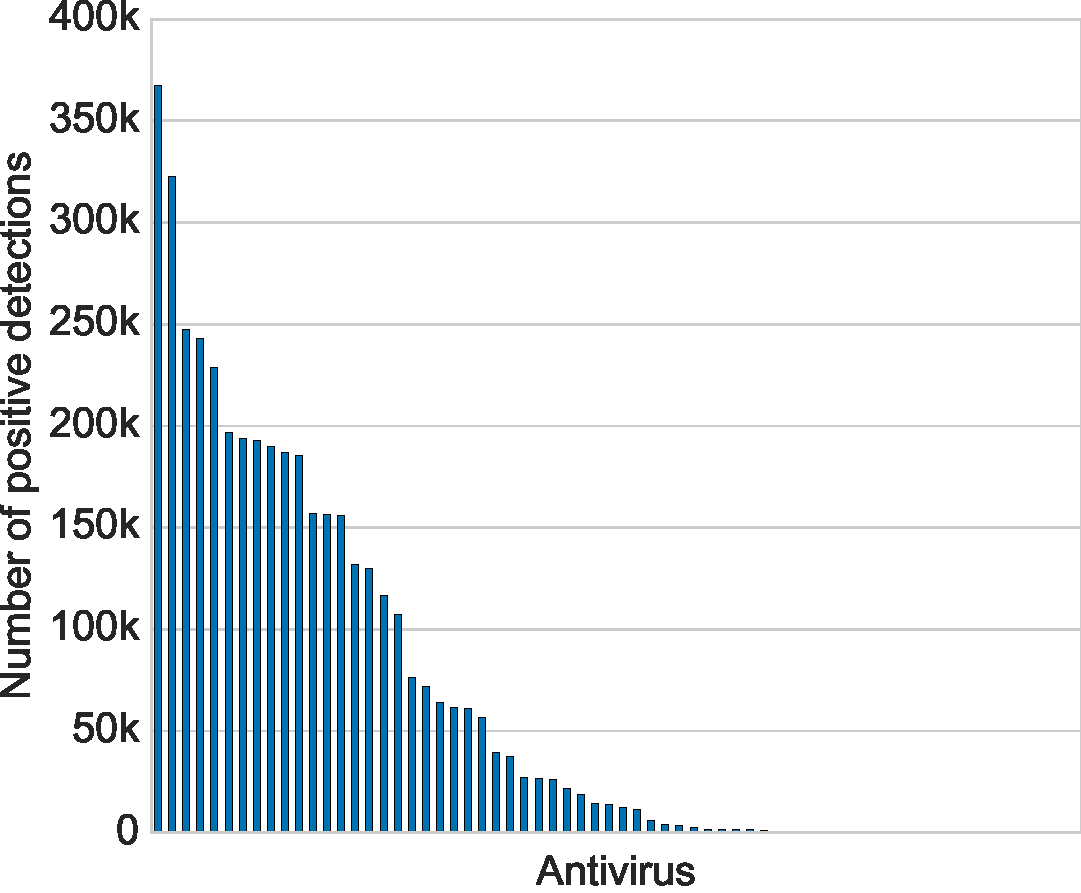
\includegraphics[width=0.75\linewidth]{figures/stase/equiponderance.pdf}
        \caption[Positive detections by antivirus]{Positive detections by antivirus in $\mathcal{D}_{base}$}
	\label{figure:stase:equiponderance}
\end{figure}

Figure~\ref{figure:stase:equiponderance} highlights the uneven distribution of positive detections per antivirus in the $\mathcal{D}_{base}$ baseline ground truth.
The number of detected applications indeed ranges from 0 to 367\,435.
This problem raises the question of the confidence in a ground truth when only antiviruses from the head and tail of the distribution contribute to the decision process.
Indeed, although we cannot assume that antivirus engines with high (or low) detection rates have better performances, because of their potential false positives (or false negatives), it is essential to consider the detection rates of antivirus for a given dataset to allow comparisons on common ground.
A corollary concern is then to characterize the ground truth to allow comparisons.
To generalize and quantify this characteristic of ground truth datasets, we consider the following research question:

\begin{mdframed}[roundcorner=10pt,nobreak=true]
	{\em Research question 1: Given a set of antivirus and the ground truth that they produce together, Is the resulting ground truth dominated by only a few antiviruses, or do all antivirus contribute the same amount of information?}
\end{mdframed}

We answer this research question with a single metric, \emph{Equiponderance}, which measures how balanced or how imbalanced are the contributions of each antivirus.
Considering our baseline settings with all antivirus engines, we infer that 9, i.e., 13.5\%, antivirus provided as many positive detections as all the other antivirus combined.
The {\em Equiponderance} aims to capture this percentage in its output.
Because the maximum value for this percentage is 50\%\footnote{If one set of antivirus leads to a percentage x over 50\%, then the other set relevant value is 100-x\% < 50\%.}, we weigh this percentage, by multiplying it by 2, to yield a metric between 0 and 1.
We define the function $Ouroboros$~\cite{hurier_definition_nodate} which computes this value and also returns the corresponding number of antiviruses, which we refer to as the Index of the {\em Equiponderance}.

\begin{mdframed}[hidealllines=true,nobreak=true]
\begin{gather*}
	Equiponderance(\mathcal{B}) = Ouroboros(X) \text{ with } X = \{positives(C_j) : C_j \in \mathcal{B}, 1 \leq j \leq n\}
\end{gather*}

\begin{itemize}
	\item{\textbf{Interpretation}} -- the minimal proportion of antivirus that detected at least 50\% applications in the dataset. The metric value is weighted.
	\item{\textbf{Minimum}:} 0 -- when a single antivirus made all the positive detections
	\item{\textbf{Maximum}:} 1 -- when the distribution of detection rates is perfectly even
\end{itemize}
\end{mdframed}

When the \emph{Equiponderance} is close to zero, the ground truth analyzed is dominated by extreme cases: a large number of antivirus engines provide only a few positive detections, while only a few antivirus engines provide most positive detections.
In comparison with $\mathcal{D}_{base}$'s {\em Equiponderance} value of 0.27, $\mathcal{D}_{genome}$ and $\mathcal{D}_{filtered}$ present \emph{Equiponderance} values of 0.48 and 0.59 respectively.
\subsection{Exclusivity}
Even in the case where several antiviruses would have the same number of detections, it does not imply any agreement of antivirus.
It is thus crucial to also quantify to what extent each antivirus tends to detect samples that no other antivirus detects.

\begin{figure}[!ht]
	\centering
	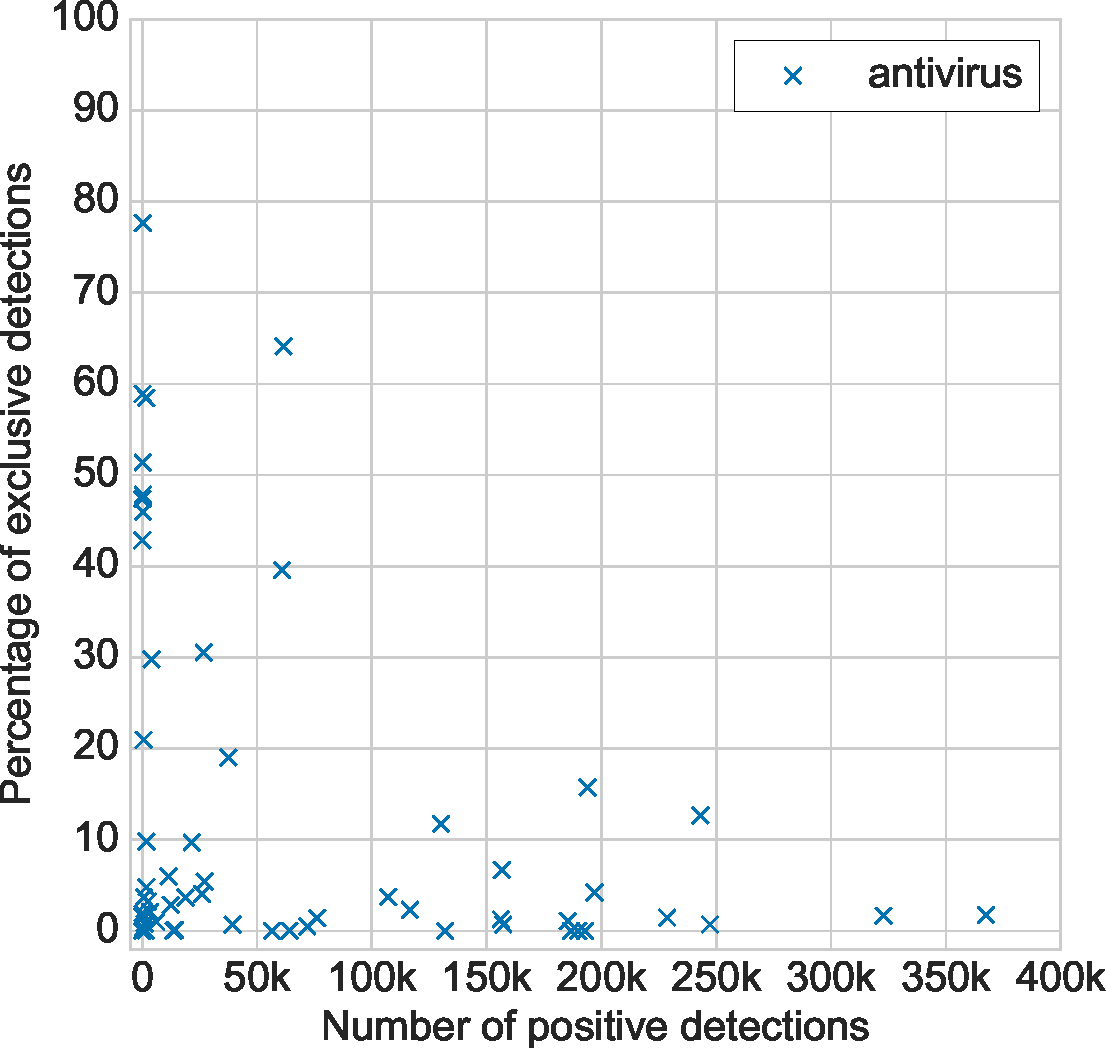
\includegraphics[width=0.75\linewidth]{figures/stase/exclusivity.pdf}
        \caption[Relation between positive and exclusive detections]{Relation between positive and exclusive detections in $\mathcal{D}_{base} $}
	\label{figure:stase:exclusivity}
\end{figure}

Figure~\ref{figure:stase:exclusivity} plots, for every antivirus product, the proportion of exclusive detections (i.e., samples no other antivirus detects) over the total number of positive detection of this antivirus.
Five antiviruses provide a majority of exclusive detections while a large part of other antivirus (45) provides less than 10\% such detections.
For the 21 antiviruses that made the most positive detections, the proportion of exclusive detections remains below 16\%, while the highest ratios of exclusive detections are associated with an antivirus that made a (relatively) small number of positive detections.
Figure~\ref{figure:stase:exclusivity} provides a important insight into Android malware detection by antivirus: A very high absolute number of detections comes from adding more non-exclusive detections, not from detecting applications no other antivirus detects as could have been intuitively expected.
The following research question aims at formally characterizing this bias in datasets:

\begin{mdframed}[roundcorner=10pt,nobreak=true]
	{\em Research question 2: Given a set of antivirus and the ground truth that they produce together, what is the proportion of samples that were included only due to one antivirus engine?}
\end{mdframed}

To answer this research question, we propose the {\em Exclusivity} metric, which measures the proportion of a tentative ground truth that is specific to a single detector.

\begin{mdframed}[hidealllines=true,nobreak=true]
\begin{gather*}
	Exclusivity(\mathcal{B}) = \dfrac{exclusives(\mathcal{B})}{m} \\
\end{gather*}

\begin{itemize}
	\item{\textbf{Interpretation}} -- the proportion of applications detected by only one
	      antivirus
	\item{\textbf{Minimum}}: 0 -- when every sample has been detected by more than one antivirus
	\item{\textbf{Maximum}}: 1 -- when every sample has been detected by only one
	      antivirus
\end{itemize}
\end{mdframed}

In $\mathcal{D}_{base}$, 31\% of applications were detected exclusively by only one antivirus, leading to an {\em Exclusivity} value of 0.31.
On the contrary, both $\mathcal{D}_{genome}$ and $\mathcal{D}_{filtered}$ do not include applications detected by only one antivirus and have an \emph{Exclusivity} of 0.
\subsection{Recognition}
Because \emph{Equiponderance} and \emph{Exclusivity} alone are not sufficient to describe how experimental ground truth datasets are built, we investigate the impact of the threshold parameter often used in the literature about malware detection to consolidate the value of positive detections~\cite{arp_drebin:_2014}.
A threshold $\tau$ indicates that a sample is considered as malware in the ground truth if and only if at least $\tau$ antivirus engines have reported positive detections on it.
Unfortunately, to the best of our knowledge, there is no theory or golden rule behind the selection of $\tau$.
On the one hand, it should be noted that samples rejected because of a threshold requirement may be either (a) new malware samples not yet recognized by all industry players, or (b) difficult cases of malware whose patterns are not easily spotted~\cite{kantchelian_better_2015}.
On the other hand, when a sample detected by $\lambda$ or $\gamma$ antivirus (where $\lambda$ is close to $\tau$ and $\gamma$ is much bigger than $\tau$), the confidence of including the application in the malware set is not equivalent for both cases.

\begin{figure}[!ht]
	\centering
	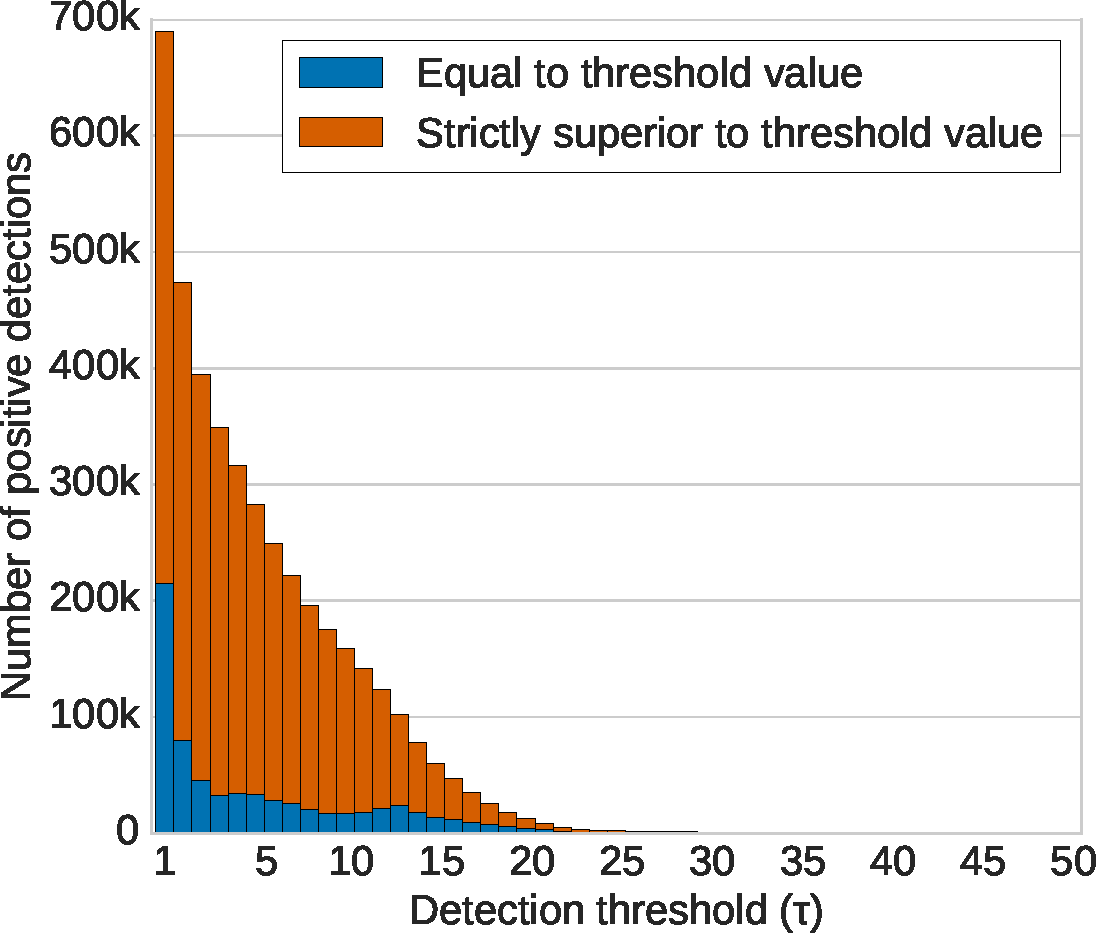
\includegraphics[width=0.75\linewidth]{figures/stase/recognition.pdf}
        \caption[Distribution of applications flagged by antivirus]{Distribution of applications flagged by $\tau$ antivirus in $\mathcal{D}_{base}$}
	\label{figure:stase:recognition}
\end{figure}

Figure~\ref{figure:stase:recognition} explores the variations in the numbers of applications included in the ground truth dataset $\mathcal{D}_{base}$ as malware when the threshold value for detection rates (i.e., threshold number $\tau$ of antivirus assigning a positive detection a sample) changes.
We also provide the number of applications detected by more than $\tau$ antivirus for the different values of $\tau$.

Both bar plots appear to be right skewed, with far more samples detected by a small number of antiviruses than by the majority of them.
Thus, any threshold value applied to this dataset would remove a large portion of the potential malware set (and, in some settings, shift them into the benign set).
To quantify this property of ground truth datasets, we investigate the following research question:

\begin{mdframed}[roundcorner=10pt,nobreak=true]
	{\em Research question 3: Given the result of antivirus scans on the ground truth dataset, have applications been marginally or widely recognized to be malicious?}
\end{mdframed}

We answer this Research question with a single metric, {\em Recognition}, which computes the average number of positive detections assigned to a sample.
In other words, it estimates the number of antiviruses agreeing on a given app.

\begin{mdframed}[hidealllines=true,nobreak=true]
\begin{gather*}
	Recognition(\mathcal{B}) = \dfrac{\sum^m_{i=1} X_i}{n \times m} \text{ with }
	X = \{positives(R_i) : R_i \in \mathcal{B}, 1 \leq i \leq m\}
\end{gather*}

\begin{itemize}
	\item{\textbf{Interpretation}} -- the proportion of antivirus which provided a positive detection to an application, averaging on the entire dataset
	\item{\textbf{Minimum}}: 0 -- when no detections were provided at all
	\item{\textbf{Maximum}}: 1 -- when each antivirus have agreed to flag all applications
\end{itemize}
\end{mdframed}

When a threshold is applied to an experimental dataset, the desired objective is often to increase the confidence by ensuring that malware samples are widely recognized to be malicious by existing antivirus engines.
Although researchers often report the effect on the dataset size, they do not measure the level of confidence that was reached.
As an example, the \emph{Recognition} of $\mathcal{D}_{base}$ is 0.09: on average, 6 (9\%) antivirus engines provided positive detections per sample, suggesting a marginal recognition by antivirus.
The \emph{Recognition} values for $\mathcal{D}_{filtered}$ and $\mathcal{D}_{genome}$ amounts to 0.36 and 0.48 respectively.
These values characterize the datasets by estimating the extent to which antivirus agree more to recognize samples from $\mathcal{D}_{filtered}$ as positive detections more widely than in $\mathcal{D}_{base}$.
Antivirus recognize samples from $\mathcal{D}_{genome}$ even more widely.
\subsection{Synchronicity}
In complement to \emph{Recognition} and \emph{Exclusivity}, we investigate the scenarios where pairs of antivirus engines conflict in their detection decisions.
Let us consider two antivirus engines $U$ and $V$ and the result of their detections on a fixed set of samples.
For each sample, we can expect 4 cases:

\newcommand{\myt}{\texttt{True}}
\newcommand{\myf}{\texttt{False}}
\begin{center}
	\begin{tabular}{lclc}
		                    & Detected by $U$ &  & Not detected by $U$ \\
		Detected By $V$     & (\myt, \myt)    &  & (\myt, \myf)        \\
		Not detected by $V$ & (\myf, \myt)    &  & (\myf, \myf)
	\end{tabular}%
\end{center}

Even if the \emph{Equiponderance} value of the dataset produced by antivirus $U$ and $V$ amounts to 1, one cannot conclude on the distribution of those cases.
The most extreme scenarios could be 50\% (True, True) and 50\% (False, False) or 50\% (True, False) and 50\% (False, True).
For the first one, both antiviruses are in perfect synchrony while they are in perfect asynchrony in the second one.

\begin{figure}[!ht]
	\centering
	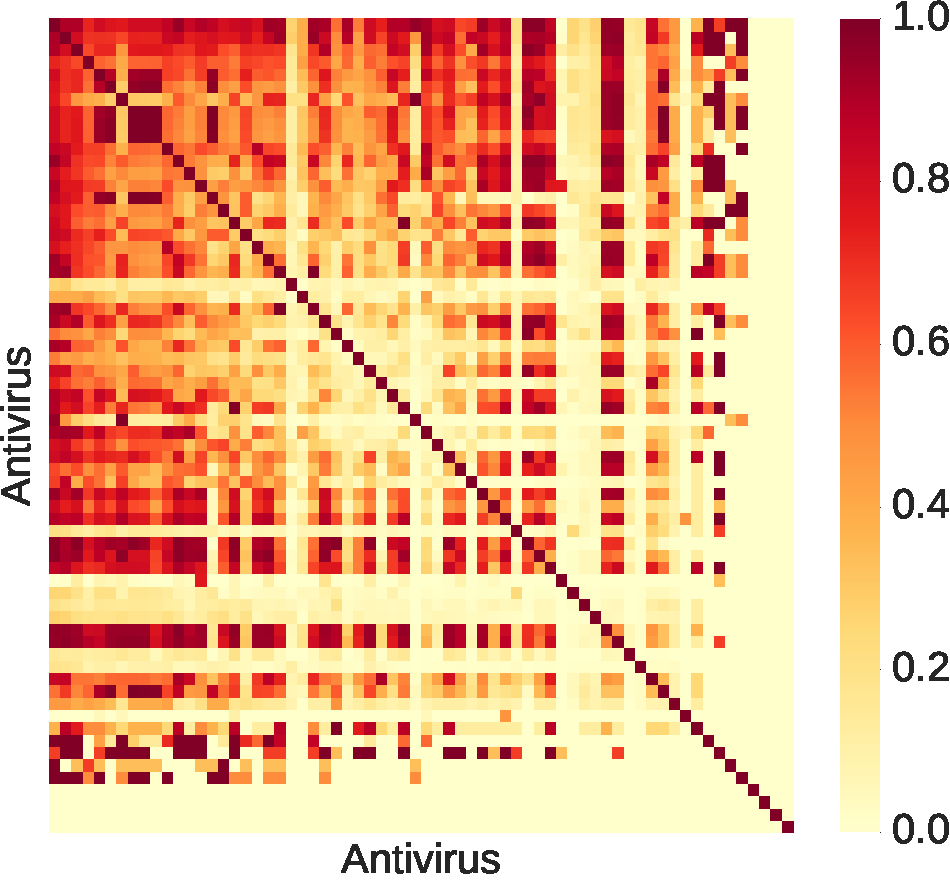
\includegraphics[width=0.75\linewidth]{figures/stase/synchronicity.pdf}
        \caption[Overlap between pairs of antivirus]{Overlap between pairs of antivirus in $\mathcal{D}_{base}$}
	\label{figure:stase:synchronicity}
\end{figure}

Figure~\ref{figure:stase:synchronicity} is a heat map representation of the pairwise agreement among the 66 antivirus engines on our dataset.
For simplicity, we have ordered the antivirus engines by their number of positive detections (the top row left to right and the left column top to bottom correspond to the same antivirus).
For each of the $\binom{66}{2}$ entries, we compute the $overlap$ function~\cite{pfitzner_characterization_2009}: $overlap(X,Y) = |X \cap Y| / \min(|X|, |Y|)$.
This function normalizes the pairwise comparison with the case of the antivirus presenting the smallest number of positive detections.
From the heat map, we can observe two patterns: (a) The number of cells where a full similarity is achieved is relatively small with respect to the number of entries.
Only 12\% of pairs of antivirus achieved a pairwise similarity superior to 0.8, and only 1\% of pairs presented a perfect similarity.
(b) There is no continuity from right to left (nor from top to bottom) of the map.
These observations indicate that antiviruses with an equal number of positive detections do not necessarily detect the same samples.
We aim to quantify this level of agreement through the following research question:

\begin{mdframed}[roundcorner=10pt,nobreak=true]
        {\em Research question 4: Given a dataset of samples and a set of antivirus, what is the likelihood for any pair of distinct antivirus engines to agree on a given sample?}
\end{mdframed}

We answer this research question with the \emph{Synchronicity} metric which measures the tendency of a set of antivirus to provide positive detections at the same time as other antivirus in the set:

\begin{mdframed}[hidealllines=true,nobreak=true]
\begin{gather*}
	Synchronicity(\mathcal{B}) = \dfrac{\sum^n_{j=1} \sum^{n}_{j'=1}
	PairwiseSimilarity(C_j, C_{j'})}{n (n-1)} \text{ with }
	j \neq j', C_j \in \mathcal{B}, C_{j'} \in \mathcal{B}
\end{gather*}

\begin{itemize}
	\item{\textbf{Interpretation}} -- average pairwise similarity between pairs of antivirus
	\item{\textbf{Minimum}}: 0 -- when no sample is detected at the same time by more~than~one~antivirus
	\item{\textbf{Maximum}}: 1 -- when each sample is detected by every antivirus
	\item{\textbf{Parameters}}
	      \begin{itemize}
		      \item{$PairwiseSimilarity$}: a binary distance function~\cite{pfitzner_characterization_2009}
		            \begin{itemize}
			            \item{Overlap}: based on positive detections and normalized (default)
			            \item{Jaccard}: based on positive detections, but not normalized
			            \item{Rand}: based on positive and negative detections
		            \end{itemize}
	      \end{itemize}
\end{itemize}
\end{mdframed}

High values of \emph{Synchronicity} should be expected for datasets where no uncertainty remains to recognize applications as either malicious or not malicious.
$\mathcal{D}_{base}$ presents a \emph{Synchronicity} of 0.32, which is lower than values for $\mathcal{D}_{genome}$ (0.41), and $\mathcal{D}_{filtered}$ (0.75).
The gap between values for $\mathcal{D}_{genome}$ and $\mathcal{D}_{filtered}$ suggests the impact that a selection of Antivirus can have on artificially increasing the \emph{Synchronicity} of the dataset.
\section{Analysis of antivirus labeling}
Besides binary decisions on detection of maliciousness in a sample, antivirus engines also provide, in case of a positive detection, a string label that indicates the type/family/behavior of the malware and identifies the malicious traits.
These labels are thus expected to specify the threat appropriately and in a meaningful and consistent way.
Nevertheless, previous works have found that the disagreement of many antiviruses on labeling a sample malware challenges their practical use~\cite{kruegel_automated_2007,canto_large_2017,jajodia_finding_2011,hutchison_av-meter:_2014}.

In this section, we further investigate the inconsistencies of malware labels and quantify different dimensions of disagreements in ground truth settings.
\subsection{Uniformity}

\begin{figure}[!ht]
        \centering
	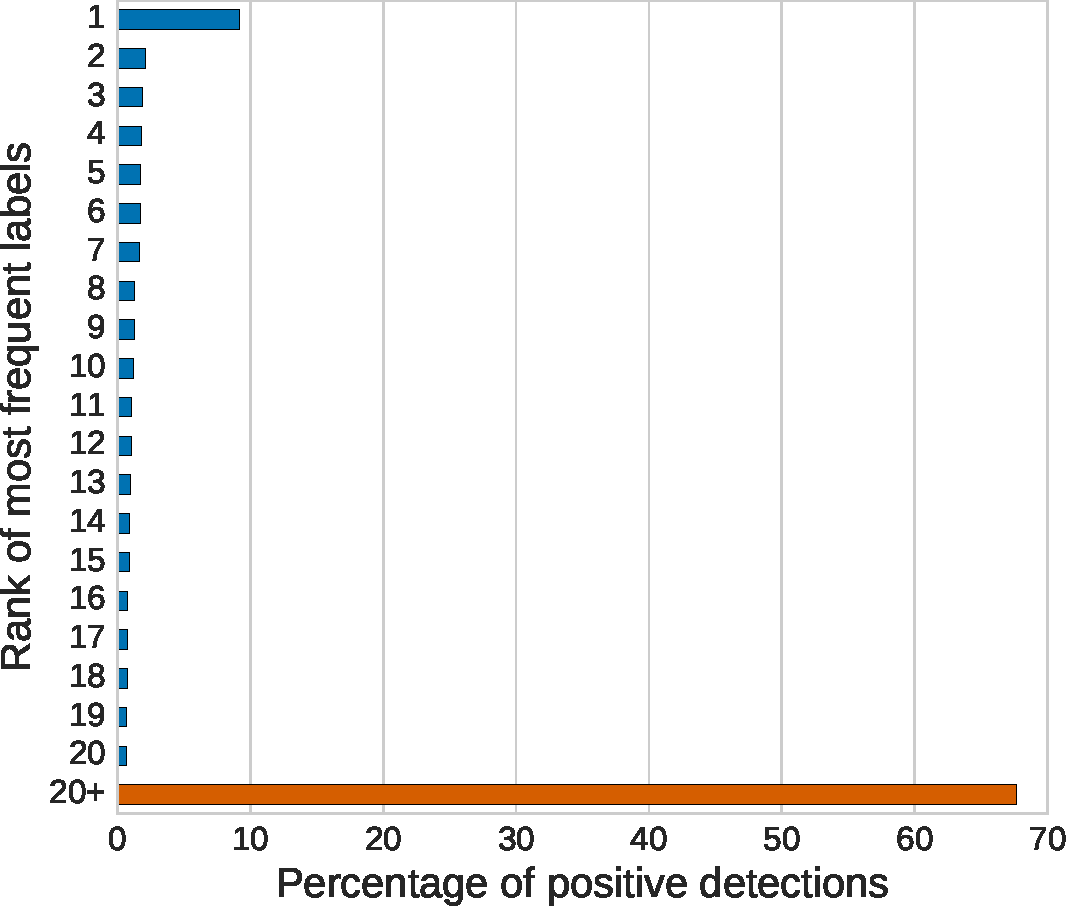
\includegraphics[width=0.75\linewidth]{figures/stase/uniformity.pdf}
        \caption[Distribution of malware labels]{Distribution of malware labels in $\mathcal{D}_{base}$}
	\label{figure:stase:uniformity}
\end{figure}

Figure~\ref{figure:stase:uniformity} represents the distribution of the most frequently used labels on our $\mathcal{D}_{base}$ dataset.
In total, the 689\,209 samples detected by at least one antivirus were labeled with 119\,156 distinct labels.

68\% of positive detections were associated with the most infrequent labels, i.e., outside the top 20 labels (grouped under the OTHERS label).
The most frequent label, \\ \texttt{Android.Adware.Dowgin.I}, is associated with 9\% of the positive detections.
In a ground truth dataset, it is essential to estimate the balance between different malicious traits, to ensure that the reported performance of an automated detector can generalize.
We assess this property of ground truth by answering the following research question:

\begin{mdframed}[roundcorner=10pt,nobreak]
	{\em Research question 5: Given a ground truth derived by leveraging a set of antivirus, are the labels associated with samples evenly distributed?}
\end{mdframed}

We answer this research question with a single metric, \emph{Uniformity}, which measures how balanced or how imbalanced are the clusters of samples associated with the different labels.

\begin{mdframed}[hidealllines=true,nobreak=true]
\begin{gather*}
	Uniformity(\mathcal{L'}) = Ouroboros(X) \text{ with }
	X = \{clusters(l_k) : l_k \in \mathcal{L'}, 1 \leq k \leq o\}
\end{gather*}

\begin{itemize}
	\item{\textbf{Interpretation}} -- minimal proportion of labels assigned to at least 50\% of the total number of detected samples. The metric value is weighted
	\item{\textbf{Minimum}}: 0 -- when each sample is assigned a unique label by each antivirus
	\item{\textbf{Maximum}}: 1 -- when the same label is assigned to every sample by all antivirus
\end{itemize}
\end{mdframed}

The \emph{Uniformity} metric is important as it may hint on whether some malware families are undersampled with respect to others in the ground truth.
In can thus help, to some extent, to quantify potential biases due to malware family imbalance.
$\mathcal{D}_{base}$ exhibits a \emph{Uniformity} value close to 0 ($12\times10^{-4}$) with an index of 75: 75 labels occur as often in the distribution than the rest of labels (119\,081), leading to uneven distribution.
We also found extreme values for both Filtered and Genome settings with \emph{Uniformity} of 0.01 and 0.04 respectively.
These values raise the question of malware families imbalance in most ground truth datasets.
However, it is possible that some labels, although distinct, because of the lack of naming standard, actually represent the same malware type.
We thus propose to examine labels on other dimensions further.
\subsection{Genericity}

\begin{figure}[!ht]
        \centering
	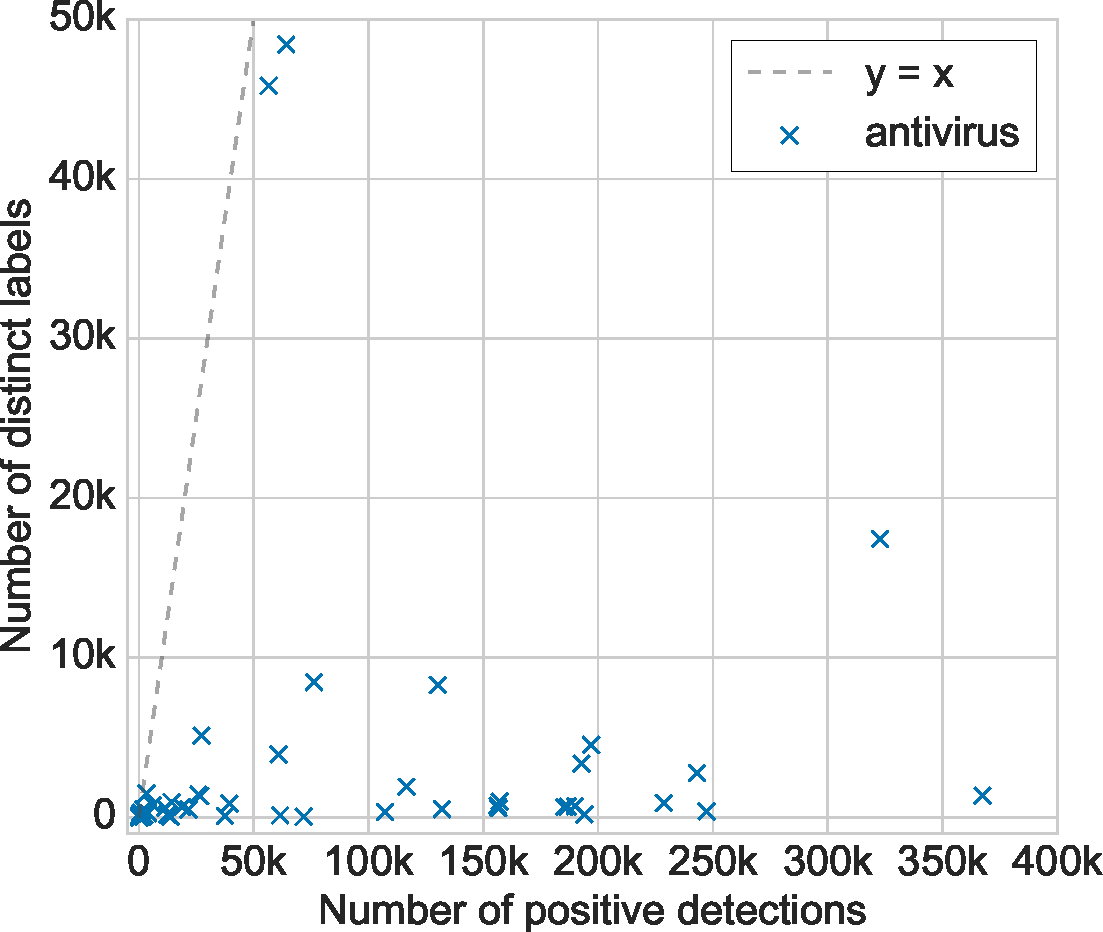
\includegraphics[width=0.75\linewidth]{figures/stase/genericity.pdf}
        \caption[Relation between distinct labels and positive detections per antivirus]{Relation between distinct labels and positive detections per antivirus in $\mathcal{D}_{base}$}
	\label{figure:stase:genericity}
\end{figure}

Once the distribution of labels has been extracted from the dataset, we can also measure how often labels are reused by antivirus.
This property is an unusual behavior that Bureau \& Harley highlighted~\cite{bureau_dose_2008}.
If we consider the two extreme cases, an antivirus could either assign a different label to every sample (e.g., hash value), or a unique label to all samples.
In both scenarios, labels would be of no value to group malware together~\cite{kruegel_automated_2007}.

In Figure~\ref{figure:stase:genericity}, we plot the number of detections against the number of distinct labels for each antivirus.
While two antiviruses assign almost a different label for each detected sample (points close to the $y=x$ line), the majority of antivirus have much fewer distinct labels than detected samples: they reuse labels amongst several samples.
Different levels of labels genericity might explain these two different behaviors
For example, using exact labels would make the sharing of labels among samples harder than in the case of generic labels that could each be shared by several samples.

To quantify this characteristic of labels produced by a set of antivirus contributing to define a ground truth, we raise the following research question:

\begin{mdframed}[roundcorner=10pt,nobreak]
	{\em Research question 6: Given a ground truth derived by leveraging a set of antivirus, what is, on average for an antivirus, the degree of reuse of a label to characterize several samples?}
\end{mdframed}

We propose the \emph{genericity} metric to quantify this information:

\begin{mdframed}[hidealllines=true,nobreak=true]
\begin{gather*}
	Genericity(\mathcal{L}) = 1 - \dfrac{o - 1}{positives(\mathcal{L}) - 1} \text{with $o \leftarrow$ number of distinct labels}
\end{gather*}

\begin{itemize}
	\item{\textbf{Interpretation}} -- the ratio between the number of distinct labels and the number of positive detections
	\item{\textbf{Minimum}}: 0 -- when every assigned label is unique
	\item{\textbf{Maximum}}: 1 -- when all labels are identical
\end{itemize}
\end{mdframed}

\emph{Genericity} assesses whether an antivirus assigns precise labels or generic ones to samples.
Although detectors with low \emph{Genericity} would appear to be more precise in their naming, Bureau \& Harley~\cite{bureau_dose_2008} support that such engines may not be the most appropriate concerning the exponential growth of malware variants.

The \emph{Genericity} $\mathcal{D}_{base}$ is 0.97, in line with our visual observation that there are far less distinct labels than positive detections.
The \emph{Genericity} values of $\mathcal{D}_{genome}$ and $\mathcal{D}_{filtered}$ are equal to 0.82 and 0.87 respectively.
\subsection{Divergence}

\begin{figure}[!ht]
        \centering
	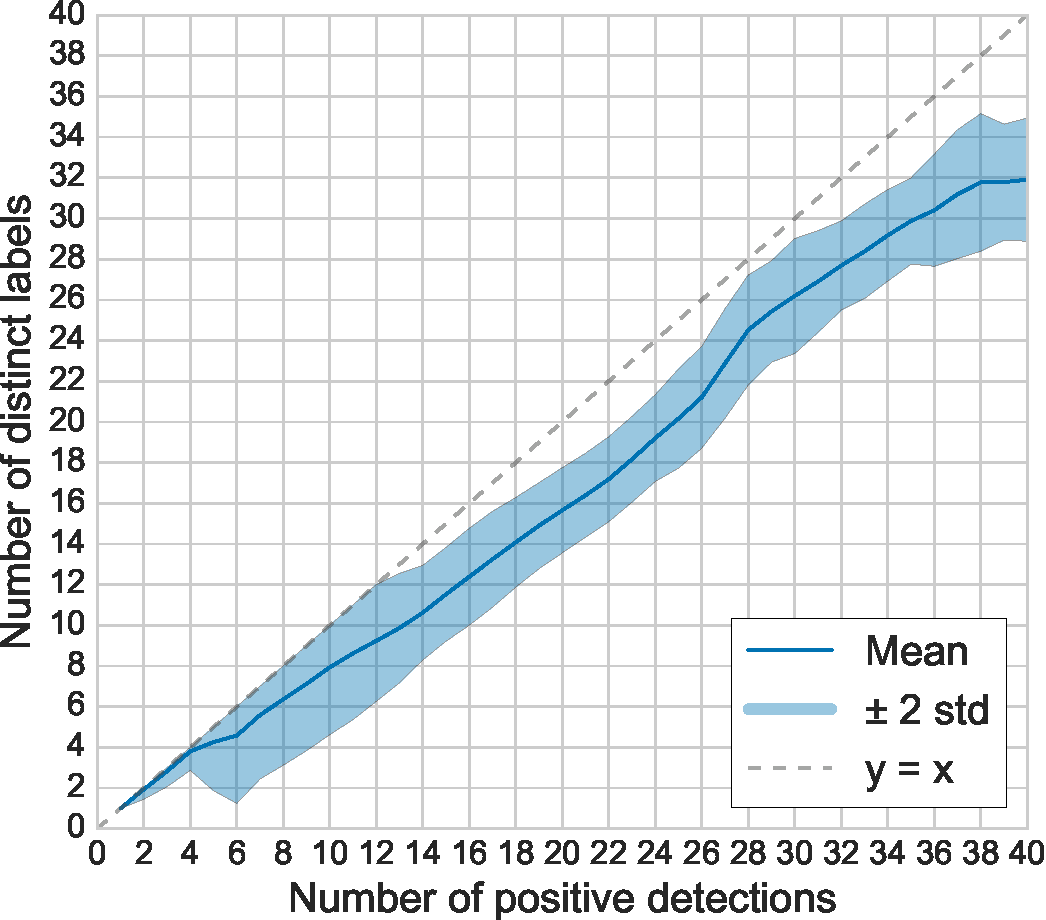
\includegraphics[width=0.75\linewidth]{figures/stase/divergence.pdf}
        \caption[Relation between distinct labels and positive detections per application]{Relation between distinct labels and positive detections per application in $\mathcal{D}_{base}$}
	\label{figure:stase:divergence}
\end{figure}

While \emph{Uniformity} and \emph{Genericity} can evaluate the overall distribution of labels that were assigned by antivirus, they do not consider the question of agreement of antivirus on each sample.
Ideally, antiviruses should be consistent and provide labels similar to that of their peers.
Even if this ideal case cannot be achieved, the number of distinct labels per application should remain limited to the number of antiviruses agreeing to detect it.

For $\mathcal{D}_{base}$, Figure~\ref{figure:stase:divergence} plots the relationship between the number of positive detections of a sample and the average number of distinct labels associated with it.
As a confidence margin, we also draw an area of two standard deviations centered on the mean.
We note that the mean value for the number of labels grows steadily with the number of detection, close to the maximum possible values represented by the dotted line.
The Pearson correlation coefficient $\rho$ between these variables evaluates to $0.98$, indicating a strong correlation.
Overall, the results suggest not only that there is a high number of different labels per application on our dataset, but also that this behavior is real for both small and high values of positive detections.
The following research question investigates this characteristic of ground truth datasets:

\begin{mdframed}[roundcorner=10pt,nobreak]
	{\em Research question 7: Given a set of antivirus and the ground truth that they produce, to what extent do antivirus provide for each sample a label that is inconsistent regarding other antivirus labels}
\end{mdframed}

We can quantify this factor with the following metric that measures the capacity of a set of antivirus to assign a high number of different labels per application.

\begin{mdframed}[hidealllines=true,nobreak=true]
\begin{gather*}
	Divergence(\mathcal{L}) = \dfrac{(\sum_{i=1}^m X_i) - n}{positives(\mathcal{L}) - n} \text{ with }
	X = \{distincts(R_i) : R_i \in \mathcal{L}, 1 \leq i \leq m\}
\end{gather*}

\begin{itemize}
	\item{\textbf{Interpretation}}: -- the average proportion of distinct labels per application with respect to the number of antiviruses providing positive detection flags
	\item{\textbf{Minimum}}: 0 -- when antivirus assign a single label to each application
	\item{\textbf{Maximum}}: 1 -- when each antivirus assigns its label to each application
\end{itemize}
\end{mdframed}

Two conditions must be met in a ground truth dataset to reach a low \emph{Divergence}: antivirus must apply the same syntax consistently for each label, and they should refer to a common semantics when mapping labels with malicious behaviors/types.
If label syntax is not consistent within the dataset, then the semantics cannot be assessed via the \emph{Divergence} metric.

The \emph{Divergence} values of $\mathcal{D}_{base}$, $\mathcal{D}_{filtered}$ and $\mathcal{D}_{genome}$ are 0.77, 0.87 and 0.95 respectively.
These results are counter-intuitive since they suggest that more constrained settings create more disagreement among antivirus in terms of labeling.
\subsection{Consensuality}
To complement the property highlighted by \emph{Divergence}, we can look at the most frequent label assigned per application.
Indeed, while the previous metric describes the number of distinct labels assigned per application, it does not measure the weight of each label, notably that of the most used label.
To some extent, this label could be used to infer the family and the version of the malware, e.g., if it used by a significant portion of antivirus to characterize a sample.

To visualize this information, still for $\mathcal{D}_{base}$, we create in Figure~\ref{figure:stase:consensuality} a plot similar to that of Figure~\ref{figure:stase:divergence}, looking now at the average number of occurrence of the most frequent label against the number of positive detections per application.

\begin{figure}[!ht]
        \centering
	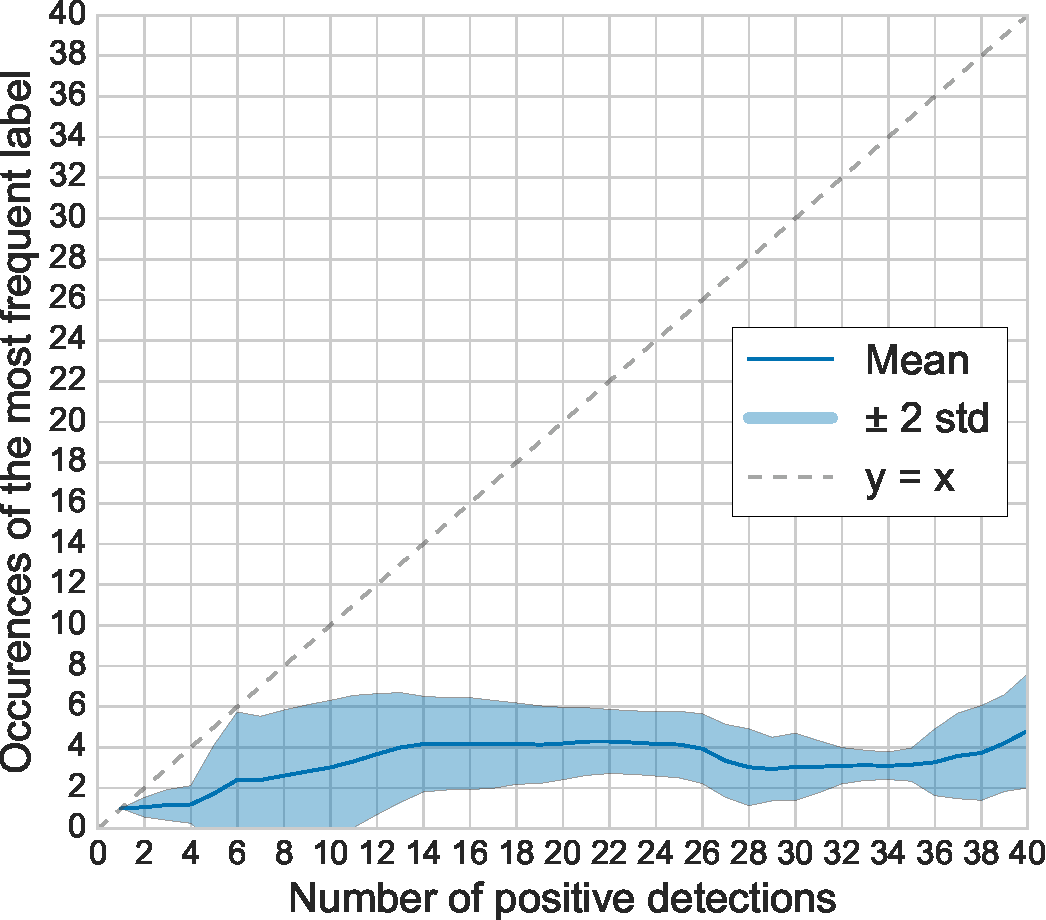
\includegraphics[width=0.75\linewidth]{figures/stase/consensuality.pdf}
        \caption[Relation between the most frequent label and positive detections per application]{Relation between the most frequent label/$\tau$ and positive detections per application in $\mathcal{D}_{base}$}
	\label{figure:stase:consensuality}
\end{figure}

The correlation coefficient $\rho$ between the two variables is $0.76$, indicative of a correlation.
Nevertheless, the relation is close to the potential minimum (x-axis).
This result is in line with our previous observations on $\mathcal{D}_{base}$ that the number of distinct labels per application was high.
The plot further highlights that the most frequent label for an application is assigned simultaneously by one to six antivirus (out of 66) on average.
This finding suggests that, at least in $\mathcal{D}_{base}$, using the most frequent label to characterize the malicious sample is not a sound approximation.
The following research question generalizes the dimension of disagreement that we investigate:

\begin{mdframed}[roundcorner=10pt,nobreak]
	{\em Research question 8: Given a set antivirus and the ground truth that they produce, to what extent can we rely on the most frequently assigned label for each detected sample as an authoritative label?}
\end{mdframed}

We answer this research question with the \emph{Consensuality} metric:

\begin{mdframed}[hidealllines=true,nobreak=true]
\begin{gather*}
	Consensuality(\mathcal{L}) = \dfrac{(\sum_{i=1}^m X_i) - n}{positives(\mathcal{L}) - n} \text{ with }
	X = \{freqmax(R_i) : R_i \in \mathcal{L}, 1 \leq i \leq m\} \\
\end{gather*}

\begin{itemize}
	\item{\textbf{Interpretation}} -- the average proportion of antivirus that agrees to assign the most frequent label. The frequency is computed per sample.
	\item{\textbf{Minimum}}: 0 -- when each antivirus assigns to each detected sample its own label (i.e., unused by others on this sample)
	\item{\textbf{Maximum}}: 1 - when all antivirus assign the same label to each sample. Different samples can have different labels however
\end{itemize}
\end{mdframed}

A high \emph{Consensuality} value highlights that the antiviruses agree on most applications to assign a most frequent label.
This metric is essential for validating, to some extent, the opportunity to summarize multiple labels into a single one.
In the $\mathcal{D}_{base}$ set, 79\% detection reports by antivirus do not come with a label that, for each sample, corresponds to the most frequent label on the sample.

The \emph{Consensuality} value of the set evaluates to 0.21.
In comparison, the \emph{Consensuality} values for $\mathcal{D}_{filtered}$ and $\mathcal{D}_{genome}$ are 0.05 and 0.06 respectively.
\subsection{Resemblance}
\emph{Divergence} and \emph{Consensuality} values on $\mathcal{D}_{base}$ suggest that labels assigned to samples cannot be used directly to represent malware families.
Indeed, the number of distinct labels per application is high (high \emph{Divergence}), and the most frequent label per application does not often occur (low \emph{Consensuality}).

We further investigate these disagreements in labels to verify whether the differences between label strings are small or large across antivirus.
Indeed, in the previous comparison, given the lack of standard naming, we have chosen to compute exact matching.
Thus, minor variations in label strings may have widely influenced our metric values.
We thus compute the similarity between label strings for each application and present the summary in Figure~\ref{figure:stase:conventionality}.

\begin{figure}[!ht]
        \centering
	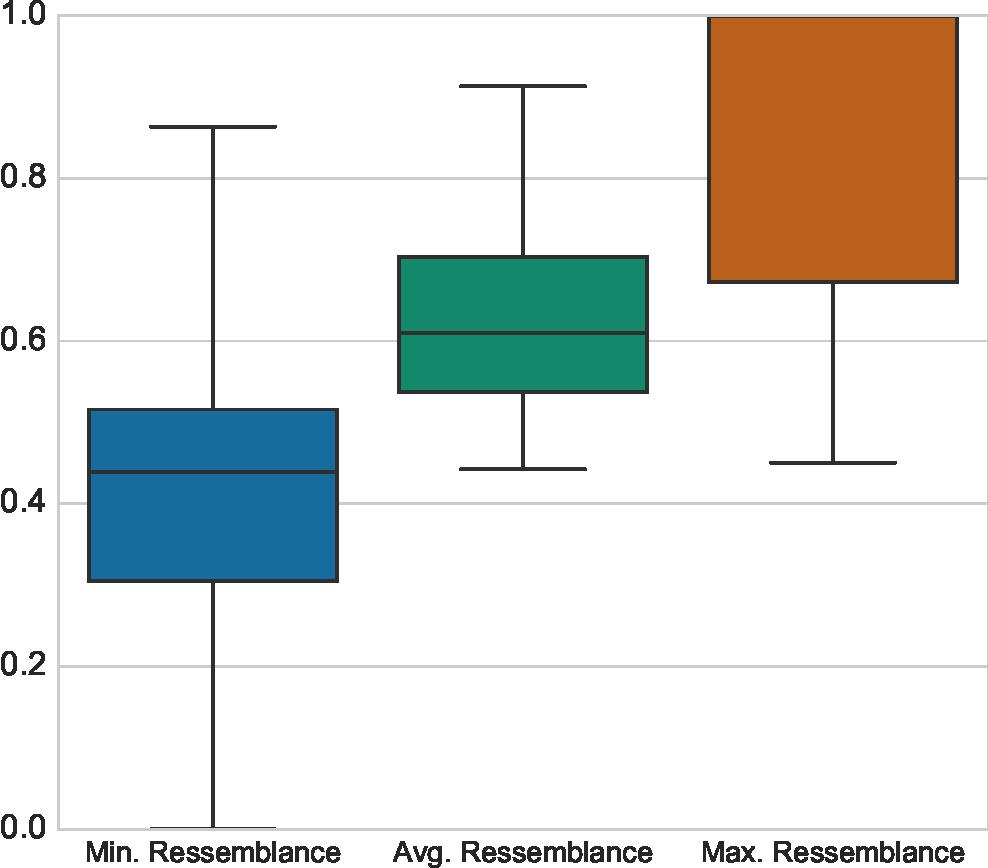
\includegraphics[width=0.75\linewidth]{figures/stase/resemblance.pdf}
        \caption[String similarity between antivirus labels per application]{String similarity between labels per application in $\mathcal{D}_{base}$}
	\label{figure:stase:conventionality}
\end{figure}

For each detected sample, we computed the Jaro-Winkler~\cite{cohen_comparison_2003} similarity between pairwise combinations of labels provided by antivirus.
This distance metric builds on the same intuition as the edit distance (i.e., Levenshtein distance), but is directly normalized between 0 and 1.
A similarity value of 1 implies the identically of strings while a value of 0 is indicative of high difference.
We consider the minimum, mean and maximum of these similarity values and represent their distributions across all applications.
The median of mean similarity values is around 0.6: on average labels only slightly resemble each other.
The following research question highlights the consensus that we attempt to measure:

\begin{mdframed}[roundcorner=10pt,nobreak]
	{\em Research question 9: Given a set antivirus and the ground truth that they produce, how resembling are the labels assigned by antivirus for each detected sample?}
\end{mdframed}

We answer this metric with the \emph{Resemblance} metric which measures the average similarity between labels assigned by a set of antivirus to a given detected sample.

\begin{mdframed}[hidealllines=true,nobreak=true]
\begin{gather*}
	Ressemblance(\mathcal{L}) = \frac{1}{m} \sum^{m}_{i=1}\dfrac{\sum^{n_i'}_{j=1} \sum^{n'_i}_{j'=1}
		Jaro-Winkler(l_{i,j}, l_{i,j'})}{n'_i (n'_i-1)} \\ \text{ with }
	j \neq j', l_{i,j} \neq \emptyset, l_{i,j'} \neq \emptyset,
	l_{i,j} \in \mathcal{B}, l_{i,j'} \in \mathcal{B} \text{ and }
	n'_i = positives(R_i), 2 \leq n_i' \leq n
\end{gather*}

\begin{itemize}
	\item{\textbf{Interpretation}} estimation of the global resemblance between labels for each app
	\item{\textbf{Minimum}} 0 when there is no similitude between labels of an application
	\item{\textbf{Maximum}} 1 when labels are identical per application
\end{itemize}
\end{mdframed}

\emph{Resemblance} assesses how labels assigned to a given application would be similar across the considered antivirus.
This metric, which is necessary when \emph{Divergence} is high and \emph{Consensuality} is low, can evaluate if the differences between label strings per application are small or large.
$\mathcal{D}_{base}$, $\mathcal{D}_{filtered}$ and $\mathcal{D}_{genome}$ present \emph{Resemblance} values of 0.63, 0.57 and 0.60 respectively.
Combined with the \emph{Divergence} metric values, we note that reducing the set of antivirus has not yielded datasets where antivirus agree more on the labels.
\section{Observations on malware datasets}
Table~\ref{table:stase:results} summarizes the metric values for the three settings described that researchers might use to build ground truth datasets.

\begin{table}[!ht]
    \caption{Summary of STASE Metrics for three common ground-truth settings}
    \label{table:stase:results}
	  \resizebox{\textwidth}{!}{  
		\begin{tabular}{|c|c|c|c|c|c|c|c|c|c|}
                \hline
		& Equiponderance & Exclusivity & Recognition & Synchronicity & Uniformity & Genericity & Divergence & Consensuality & Resemblance \\
		\hline
		$\mathcal{D}_{base}$ & 0.27 & 0.31 & 0.09 & 0.32 & 0.001 & 0.97 & 0.77 & 0.21 & 0.63 \\
		$\mathcal{D}_{filtered}$ & 0.59 & 0 & 0.36 & 0.75  & 0.01 & 0.87 & 0.95 & 0.05 & 0.57 \\
		$\mathcal{D}_{genome}$ & 0.48 & 0 & 0.48 & 0.41 & 0.04 & 0.82 & 0.87 & 0.06 & 0.60 \\
                \hline
	\end{tabular}
	}
\end{table}


The higher values of \emph{Recognition} and \emph{Synchronicity} for $\mathcal{D}_{genome}$ and $\mathcal{D}_{filtered}$ in comparison with $\mathcal{D}_{base}$ suggest that these datasets were built with samples that are well known to be malicious in the industry.
If we consider that higher \emph{Recognition} and \emph{Synchronicity} values provide guarantees for more reliable ground truth, then $\mathcal{D}_{genome}$ and $\mathcal{D}_{filtered}$ are better ground truth candidates than $\mathcal{D}_{base}$.
Their lower value of \emph{Genericity} also suggests that antivirus labels provided are more precise than those in $\mathcal{D}_{base}$.
At the same time, higher values of \emph{Equiponderance} and \emph{Uniformity} imply that both antivirus detections and labels are more balanced across antivirus.

\emph{Divergence} and \emph{Consensuality} values, however, suggest that the general agreement on antivirus labels has diminished in $\mathcal{D}_{genome}$ and $\mathcal{D}_{filtered}$ in comparison with $\mathcal{D}_{base}$.
The \emph{Exclusivity} value of 0 for $\mathcal{D}_{genome}$ and $\mathcal{D}_{filtered}$ further highlights that the constraints put on building those datasets may have eliminated corner cases of malware that only a few, if not 1, antivirus could have been able to spot.

We also note that $\mathcal{D}_{filtered}$ has a higher \emph{Synchronicity} value than $\mathcal{D}_{genome}$, indicating that its settings lead to a selection of antivirus which was more in agreement on their decision.
In contrast, the \emph{Divergence} values indicate that the proportion of distinct labels for each sample was higher in $\mathcal{D}_{filtered}$ than in $\mathcal{D}_{genome}$, suggesting that decisions in $\mathcal{D}_{genome}$ are more comfortable to interpret for each sample.
Nevertheless, the classification of samples in malware families would be more difficult because of the higher proportion of distinct labels to take into consideration.
\section{Recommendations for experiments}
In this work, we have investigated the output of antivirus systems for Android applications.
Based on different metrics, we assessed the discrepancies between three ground truth datasets, independently of their size, and question their reliability for evaluating the performance of malware experiments.
The main objective of our work is to provide means for researchers to qualify their ground truth datasets, with respect to antivirus and their heuristics, to increase confidence in research assessments.
We also believe that our work can improve the reproducibility of experimental settings, given the limited sharing of security data such as malware samples.

Besides, our analysis of antivirus reports has exposed a global lack of consensus previously highlighted by other authors on other computing platforms~\cite{kruegel_automated_2007, bureau_dose_2008, harley_game_2009, jajodia_finding_2011}.
Although our work cannot solve the challenge of naming inconsistencies directly, the metrics we propose can evaluate ground truth datasets prior and posterior to their transformation by other techniques~\cite{perdisci_vamo:_2012, wang_rebuilding_2014, kantchelian_better_2015}.
To uncover the information contained in antivirus reports, we propose that new approaches should be developed to understand the structure of malware labels and unify their output into a standard naming scheme.
